% AB=AC=AD. The angle below is a layout choice only; no angle mark is shown.
% Both circles are tangent to AD at D; M1 is tangent to AB at B and M2 to AC at C.
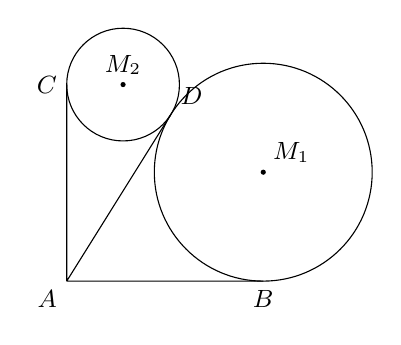
\begin{tikzpicture}[scale=0.78, every node/.style={font=\small}]
  \def\L{3.2}
  \def\theta{58}
  % 仅为安排示意图的可视位置选角；不标示意角度，不作为新增题设。
  \pgfmathsetmacro{\Dxx}{\L*cos(\theta)}
  \pgfmathsetmacro{\Dyy}{\L*sin(\theta)}
  \pgfmathsetmacro{\rOne}{\L*tan(\theta/2)}
  \pgfmathsetmacro{\rTwo}{\L*(1-sin(\theta))/cos(\theta)}

  \coordinate (A) at (0,0);
  \coordinate (B) at (\L,0);
  \coordinate (C) at (0,\L);
  \coordinate (D) at (\Dxx,\Dyy);
  \coordinate (Mone) at (\L,\rOne);
  \coordinate (Mtwo) at (\rTwo,\L);

  \draw (A) -- (B) (A) -- (C) (A) -- (D);
  \draw (Mone) circle (\rOne);
  \draw (Mtwo) circle (\rTwo);
  \fill (Mone) circle (1.2pt);
  \fill (Mtwo) circle (1.2pt);

  \node[below left] at (A) {$A$};
  \node[below] at (B) {$B$};
  \node[left] at (C) {$C$};
  \node[above right] at (D) {$D$};
  \node[above right] at (Mone) {$M_1$};
  \node[above] at (Mtwo) {$M_2$};
\end{tikzpicture}
